\documentclass[tikz,border=4pt]{standalone}
\usepackage{amsmath,amssymb}

\usetikzlibrary{arrows.meta,positioning,automata,shapes,shapes.misc,calc,decorations.pathmorphing,decorations.markings,angles,quotes,patterns,mindmap,matrix,knots,hobby,trees}
\tikzset{->-/.style={decoration={markings, mark=at position 0.5 with {\arrow{Stealth}}}, postaction={decorate}}}
\begin{document}
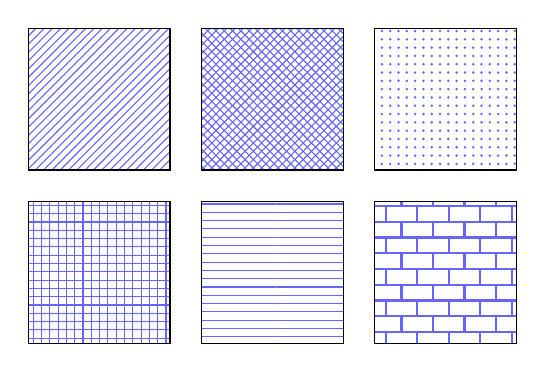
\begin{tikzpicture}
\foreach \p [count=\i] in {north east lines, crosshatch, dots, grid, horizontal lines, bricks} {
  \draw[pattern=\p, pattern color=blue!60] ({mod(\i-1,3)*2.2},{-int((\i-1)/3)*2.2}) rectangle ++(1.8,1.8);
}
\end{tikzpicture}
\end{document}
